In this section, we present the methodology and results of our evaluation, which assesses the performance of \textit{Apollon} in
traditional and AML attack environments.
The code that was used and created during the evaluation of our proposal is completely open and accessible.
It can be found on GitHub~\footnote{\url{https://github.com/antonioalfa22/apollon}}.


\subsection{Methodology}\label{subsec:methodology}
We designed two scenarios to assess the performance of our proposed solution.
In the first scenario, we tested our solution on three datasets: CIC-IDS-2017, CSE-CIC-IDS-2018, and CIC-DDoS-2019.
Due to our lack of powerful machines, we opted to use a representative subset of the datasets instead of the complete
data to efficiently train and test our models.
For the dataset CIC-DDoS-2019 the whole dataset has been used, while for the dataset CSE-CIC-IDS-2018 the subset
from \textit{02-15-2018} has been used.
Finally, for the CIC-IDS-2017 dataset, the following subsets of data have been selected:

\begin{itemize}
    \item \textit{Friday WorkingHours Afternoon DDoS}
    \item \textit{Friday WorkingHours Afternoon PortScan}
    \item \textit{Friday WorkingHours Morning}
    \item \textit{Monday WorkingHours}
    \item \textit{Thursday WorkingHours Afternoon Infilteration}
    \item \textit{Thursday WorkingHours Morning WebAttacks}
    \item \textit{Tuesday WorkingHours}
\end{itemize}


We compared the results of our solution with the classifiers extracted from related work.
In the second scenario, we used several grey/black-box Adversarial Machine Learning attacks to evaluate the ability of
our solution to defend against such attacks.

The classifiers scores used to compare our solution may be different than those reported in related work due to several
factors.
Firstly, the machine on which the training is performed may differ from that of related work.
This can impact the speed and efficiency of the training process, which in turn can affect the final accuracy of the
classifiers.
Secondly, the pre-processing of the data may be different between our solution and related work.
Pre-processing techniques can greatly impact the quality of the data and hence the performance of the classifiers.
Therefore, differences in pre-processing techniques can lead to varying levels of accuracy in the classifiers.
It is important to take into account these differences when comparing our solution to related work, and to consider
the impact of these factors on the performance of the classifiers.

All the experiments were performed on a \textit{Ubuntu 20.04.5 LTS} machine with an
\textit{Intel(R) Core(TM) i7-7700 CPU @ 3.60GHz} processor and 16 GB of RAM memory.


\subsubsection{Traditional Network Traffic and Attacks}
In this test scenario, we utilized the CIC-IDS-2017, CSE-CIC-IDS-2018, and CIC-DDoS-2019 datasets to train a set
of classifiers to compare with our proposed solution.
Our goal was to assess the performance of our solution with the traditional network traffic and web attacks.

We have utilized default hyperparameters of the classifiers because the objective of this scenario is not to
maximize the performance of these classifiers but rather to compare them with our solution.
The classifiers used in this scenario are the following:

\begin{itemize}
    \item \textit{Multilayer Perceptron (MLP)}: hidden\_layer\_sizes = (32), max\_iter = 200
    \item \textit{Random Forest (RF)}: n\_estimations = 100
    \item \textit{Decision Trees (DT)}
    \item \textit{Naive Bayes (NB)}
    \item \textit{Logistic Regression (LR)}
\end{itemize}

\subsubsection{Adversarial Machine Learning Attacks}

In this test scenario, we used several grey/black-box Adversarial Machine Learning attacks to evaluate the ability of
our solution to defend against such attacks.
To simplify the evaluation process, we used the CIC-IDS-2017 dataset to train the classifiers and our proposed solution
because it is the most popular dataset.
We compare the accuracy and the detection rate of the classifiers and our proposed solution against the grey/black-box
Adversarial Machine Learning attacks.
As we mentioned before, we only test with grey/black-box attacks because white-box attacks are not realistic in
real-world scenarios.

The attacks used in this scenario are the following:

\begin{itemize}
    \item \textit{Zeroth-order optimization attack (ZOO)}~\cite{chen2017zoo}
    \item \textit{HopSkipJump attack (HSJA)}~\cite{chen2020hopskipjumpattack}
    \item \textit{W-GAN based attacks}~\cite{lin2022idsgan}
\end{itemize}

We opted for these particular attacks because they encompass a broad spectrum of potential Adversarial Machine Learning
evasion strategies and are among the most widely used and successful.

\subsection{Results}

Throughout the development of the evaluation we have decided to set a seed, so that the results can be replicated: the \textit{seed = 42}.

Before training the classifiers, a common pre-processing step was performed on the data from all datasets.
This step is essential in standardizing the datasets, ensuring that we are working uniformly with each of them.
To achieve this, a combination of \textit{sklearn} functions such as \textit{RobustScaler} and \textit{Normalizer}
was utilized.
To make features less sensitive to outliers, the \textit{RobustScaler} subtracts the median and adjusts the data based on the quantile range.
The \textit{Normalizer} scales the input data set to have a norm of 1 and values between 0 and 1.

In addition to standardizing the datasets, additional steps were taken to further prepare the data for training our
classifiers. We avoided excessive pre-processing, to preserve as much data as possible, so we only eliminated duplicate elements and attributes that had only unique data.

We also encountered some data with missing values (\textit{NaN}) and explored various methods to handle this issue:
filling in missing values with a fixed value, with the mean or median of the feature's non-missing values,
with a prediction based on the other features and with a prediction based on k-nearest neighbors.
Our experiments revealed that using a constant value of 0 to fill in missing values achieved the best performance in the training step.

We apply this pre-processing to all datasets equally.
When validating the results we used a cross validation, in which the following parameters have been used:

\begin{itemize}
    \item n\_splits: 5
    \item test\_size: 0.2
    \item random\_state: seed
\end{itemize}
By using cross-validation we ensure that the results obtained are representative and not the result of an isolated iteration. 

The results of our experiments in the two evaluation scenarios are presented below.


\subsubsection{Traditional Network Traffic and Attacks}
In this scenario, we trained a the selected classifiers on the CIC-IDS-2017, CSE-CIC-IDS-2018, and CIC-DDoS-2019 datasets.
Additionally, we trained our proposed solution on the same datasets and with the same classifiers.
To train \textit{Apollon}, we use the K-Means~\cite{likas2003global} algorithm to cluster the data into 2 clusters.
For each cluster, we train the selected classifiers and we update the \textit{Multi-Armed Bandits} algorithm with the results.

The results obtained from the experiments are presented in the tables~\ref{tab:traditional-network-results-2017},
~\ref{tab:traditional-network-results-2018}, and~\ref{tab:traditional-network-results-2019}.
Based on the tables, our solution demonstrates high detection rate and accuracy scores, comparable to the classifiers
chosen for comparison.
It's important to mention that among all the datasets, \textit{Apollon} doesn't achieve the best or the worst scores.
This is due to the fact that \textit{Apollon} internally selects from the same classifiers.
Hence, the highest score that \textit{Apollon} can achieve is limited to the best classifier's maximum score, while it can never
perform as poorly as the worst classifier since it has other better options.

\begin{table}
    \centering
    \resizebox{\columnwidth}{!}{
        \begin{tabular}{l|lccccl|}
            \cline{2-7}
             & \multicolumn{6}{c|}{\textbf{CIC-IDS-2017}} \\ \hline
            \multicolumn{1}{|l|}{Metrics} & \multicolumn{1}{c|}{MLP} & \multicolumn{1}{c|}{NB} & \multicolumn{1}{c|}{RF} & \multicolumn{1}{c|}{DT} & \multicolumn{1}{c|}{LR} & \multicolumn{1}{c|}{\textbf{Apollon}} \\ \hline
            \multicolumn{1}{|l|}{Accuracy} & 0.9766 & 0.6694 & 0.9996 & 0.9980 & 0.9516 & \textbf{0.9740} \\
            \multicolumn{1}{|l|}{Detection rate} & 0.9731 & 0.8049 & 0.9996 & 0.9962 & 0.8360 & \textbf{0.9420} \\
            \multicolumn{1}{|l|}{F1} & 0.9760 & 0.6118 & 0.9991 & 0.9959 & 0.8858 & \textbf{0.7699} \\
            \multicolumn{1}{|l|}{ROC} & 0.9998 & 0.8289 & 1.0000 & 0.9972 & 0.9902 & \textbf{0.9420} \\ \hline
        \end{tabular}
    }
    \caption{Results of the traditional network traffic and attacks scenario on the CIC-IDS-2017 dataset.}
    \label{tab:traditional-network-results-2017}
\end{table}

\begin{table}
    \centering
    \resizebox{\columnwidth}{!}{
        \begin{tabular}{l|llllll|}
            \cline{2-7}
             & \multicolumn{6}{c|}{\textbf{CSE-CIC-IDS-2018}} \\ \hline
            \multicolumn{1}{|l|}{Metrics} & \multicolumn{1}{c|}{MLP} & \multicolumn{1}{c|}{NB} & \multicolumn{1}{c|}{RF} & \multicolumn{1}{c|}{DT} & \multicolumn{1}{c|}{LR} & \multicolumn{1}{c|}{\textbf{Apollon}} \\ \hline
            \multicolumn{1}{|l|}{Accuracy} & 0.9916 & 0.7280 & 0.9993 & 0.9939 & 0.9593 & \textbf{0.9064} \\
            \multicolumn{1}{|l|}{Detection rate} & 0.9367 & 0.8563 & 0.9967 & 0.9961 & 0.6008 & \textbf{0.9419} \\
            \multicolumn{1}{|l|}{F1} & 0.9545 & 0.5507 & 0.9963 & 0.9968 & 0.6556 & \textbf{0.7303} \\
            \multicolumn{1}{|l|}{ROC} & 0.9945 & 0.8605 & 0.9993 & 0.9984 & 0.9592 & \textbf{0.9419} \\ \hline
        \end{tabular}
    }
    \caption{Results of the traditional network traffic and attacks scenario on the CSE-CIC-IDS-2018 dataset.}
    \label{tab:traditional-network-results-2018}
\end{table}

\begin{table}
    \centering
    \resizebox{\columnwidth}{!}{
        \begin{tabular}{l|llllll|}
            \cline{2-7}
             & \multicolumn{6}{c|}{\textbf{CIC-DDoS-2019}} \\ \hline
            \multicolumn{1}{|l|}{Metrics} & \multicolumn{1}{c|}{MLP} & \multicolumn{1}{c|}{NB} & \multicolumn{1}{c|}{RF} & \multicolumn{1}{c|}{DT} & \multicolumn{1}{c|}{LR} & \multicolumn{1}{c|}{\textbf{Apollon}} \\ \hline
            \multicolumn{1}{|l|}{Accuracy} & 0.9998 & 0.9990 & 0.9999 & 0.9999 & 0.9970 & \textbf{0.9996} \\
            \multicolumn{1}{|l|}{Detection rate} & 0.8985 & 0.8709 & 0.9932 & 0.9999 & 0.7930 & \textbf{0.9691} \\
            \multicolumn{1}{|l|}{F1} & 0.9186 & 0.7148 & 0.9957 & 0.9991 & 0.8541 & \textbf{0.8521} \\
            \multicolumn{1}{|l|}{ROC} & 0.9817 & 0.9753 & 0.9999 & 0.9999 & 0.9796 & \textbf{0.9691} \\ \hline
        \end{tabular}
    }
    \caption{Results of the traditional network traffic and attacks scenario on the CIC-DDoS-2019 dataset.}
    \label{tab:traditional-network-results-2019}
\end{table}

Our results demonstrate that even with the integration of new security mechanisms, \textit{Apollon} can still provide high accuracy
and detection rate scores in traditional network traffic classification environments.
Therefore, \textit{Apollon} is capable of preserving the fundamental functionality of an IDS.

\subsubsection{Adversarial Machine Learning Attacks}
In this scenario, we have launched three types of Adversarial Machine Learning attacks on the selected classifiers and
against our solution.
These attacks are \textit{Zeroth-order optimization attack (ZOO)}, \textit{HopSkipJump attack (HSJA)} and W-GAN based attacks.

The classifiers and the \textit{Apollon} implementation used as targets of the attacks are the ones trained in the previous environment
with the CIC-IDS-2017 dataset.

Starting with the \textit{Zeroth-order optimization attack (ZOO)}, we have used the open source implementation provided by ART~\cite{art2018},
and created a Classifier class so that \textit{Apollon} can be used as a model.
The attack was launched with the following parameters for each classifier:

\begin{itemize}
    \item \textbf{classifier}: the Classifier class instance with the classifier to be attacked.
    \item targeted: True.
    \item learning\_rate: $0.01$.
    \item max\_iter: 100.
\end{itemize}

The attack was launched against the classifiers and the results are shown in Table~\ref{tab:zoo-aml-results} and in the
Figure~\ref{fig:zoo-aml-results}.
According to the findings, the attack was effective in every scenario, resulting in reduced detection rates across all classifiers.
Nonetheless, even though the \textit{Apollon} implementation's accuracy and detection rate scores also declined, they remained considerably
superior to those of the other classifiers, with high accuracy and detection rate scores.

\begin{table}
    \centering
    \resizebox{\columnwidth}{!}{
        \begin{tabular}{l|llllll|}
            \cline{2-7}
             & \multicolumn{6}{c|}{\textbf{ZOO attack}} \\ \hline
            \multicolumn{1}{|l|}{Metrics} & \multicolumn{1}{c|}{MLP} & \multicolumn{1}{c|}{NB} & \multicolumn{1}{c|}{RF} & \multicolumn{1}{c|}{DT} & \multicolumn{1}{c|}{LR} & \multicolumn{1}{c|}{\textbf{Apollon}} \\ \hline
            \multicolumn{1}{|l|}{Accuracy} & 0.7630 & 0.7160 & 0.7730 & 0.7890 & 0.5210 & \textbf{0.9304} \\
            \multicolumn{1}{|l|}{Detection rate} & 0.5260 & 0.5500 & 0.5460 & 0.5780 & 0.0420 & \textbf{0.8772} \\ \hline
        \end{tabular}
    }
    \caption{Results of the \textit{ZOO} AML attack}
    \label{tab:zoo-aml-results}
\end{table}

\begin{figure}
    \centering
    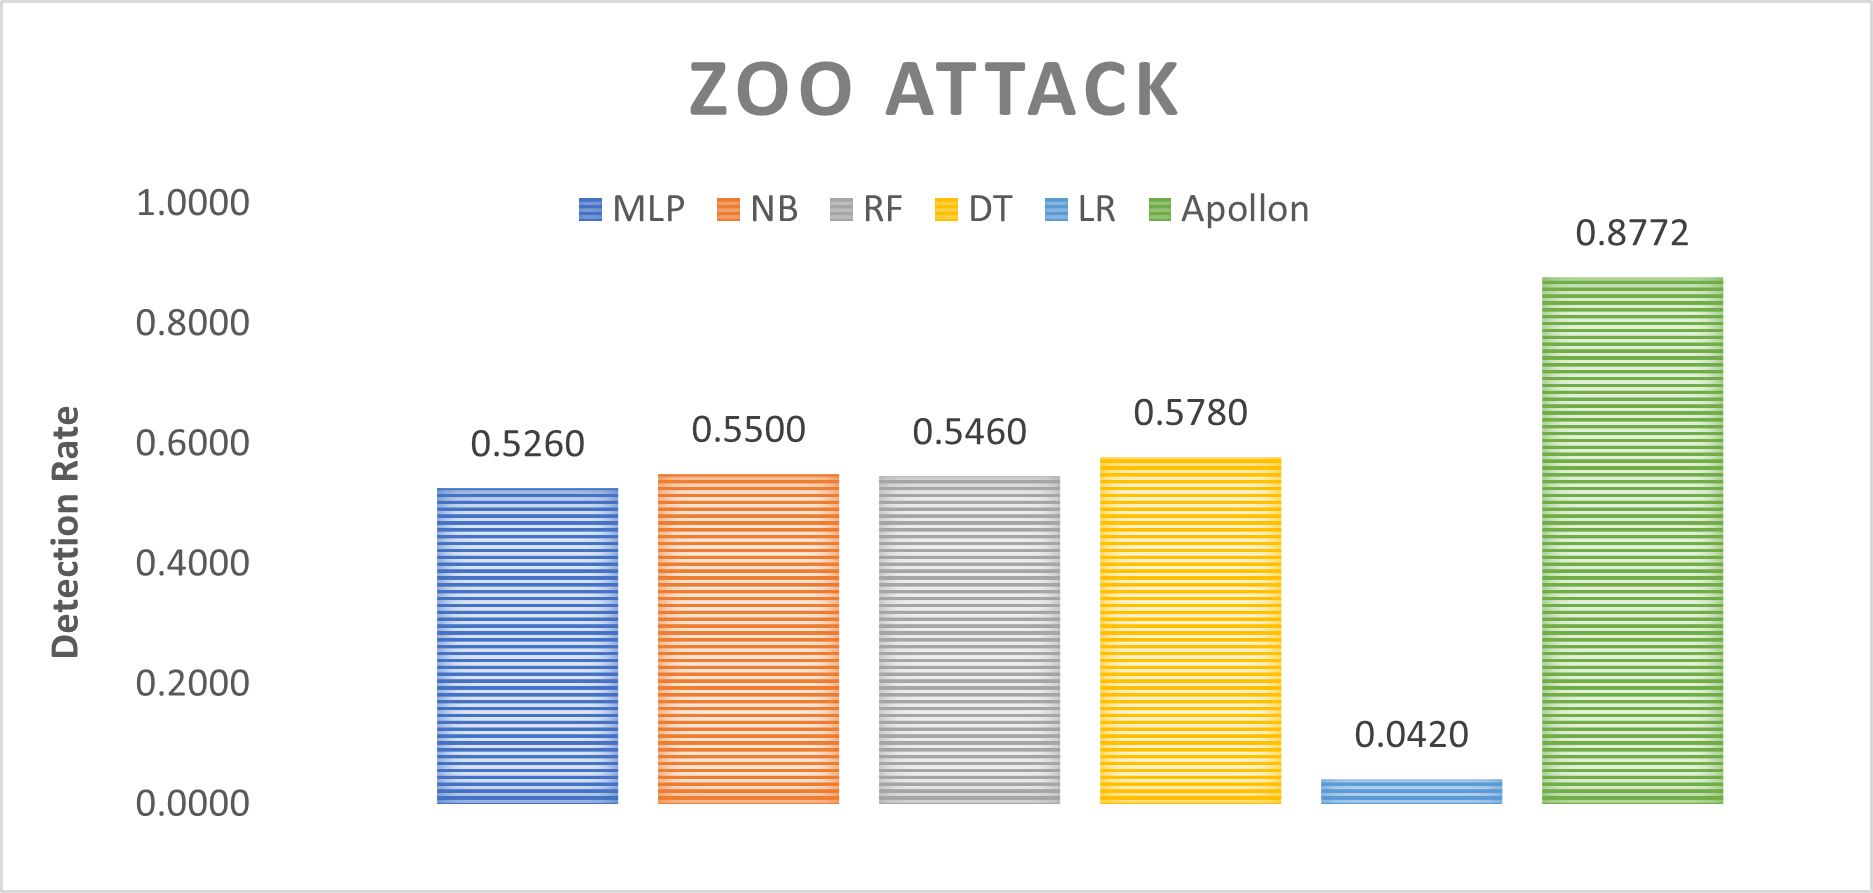
\includegraphics[width=0.9\columnwidth]{ZOO.png}
    \caption{\textit{ZOO} attack detection rate results}
    \label{fig:zoo-aml-results}
\end{figure}

To launch the \textit{HopSkipJump attack (HSJA)}, we have used the open source implementation provided by ART, and created a Classifier
as in the \textit{ZOO} attack.
The attack was launched with the following parameters for each classifier:

\begin{itemize}
    \item \textbf{classifier}: the Classifier class instance with the classifier to be attacked.
    \item targeted: True.
    \item max\_iter: 100.
    \item norm: inf.
\end{itemize}


The results of the attack are shown in Table~\ref{tab:hotskipjump-aml-results} and in the Figure~\ref{fig:hopskipjump-aml-results}.
The attack was very effective in all the classifiers, resulting in reduced detection rates to scores close to zero.
The exception was the \textit{Apollon} implementation, which was able to maintain a detection rate > 0.5.

\begin{table}
    \centering
    \resizebox{\columnwidth}{!}{
        \begin{tabular}{l|llllll|}
            \cline{2-7}
             & \multicolumn{6}{c|}{\textbf{HopSkipJump attack}} \\ \hline
            \multicolumn{1}{|l|}{Metrics} & \multicolumn{1}{c|}{MLP} & \multicolumn{1}{c|}{NB} & \multicolumn{1}{c|}{RF} & \multicolumn{1}{c|}{DT} & \multicolumn{1}{c|}{LR} & \multicolumn{1}{c|}{\textbf{Apollon}} \\ \hline
            \multicolumn{1}{|l|}{Accuracy} & 0.5002 & 0.4301 & 0.5001 & 0.5051 & 0.5900 & \textbf{0.7550} \\
            \multicolumn{1}{|l|}{Detection Rate} & 0.0000 & 0.0000 & 0.0000 & 0.0100 & 0.1800 & \textbf{0.5260} \\ \hline
        \end{tabular}
    }
    \caption{Results of the \textit{HopSkipJump} AML attack}
    \label{tab:hotskipjump-aml-results}
\end{table}

\begin{figure}
    \centering
    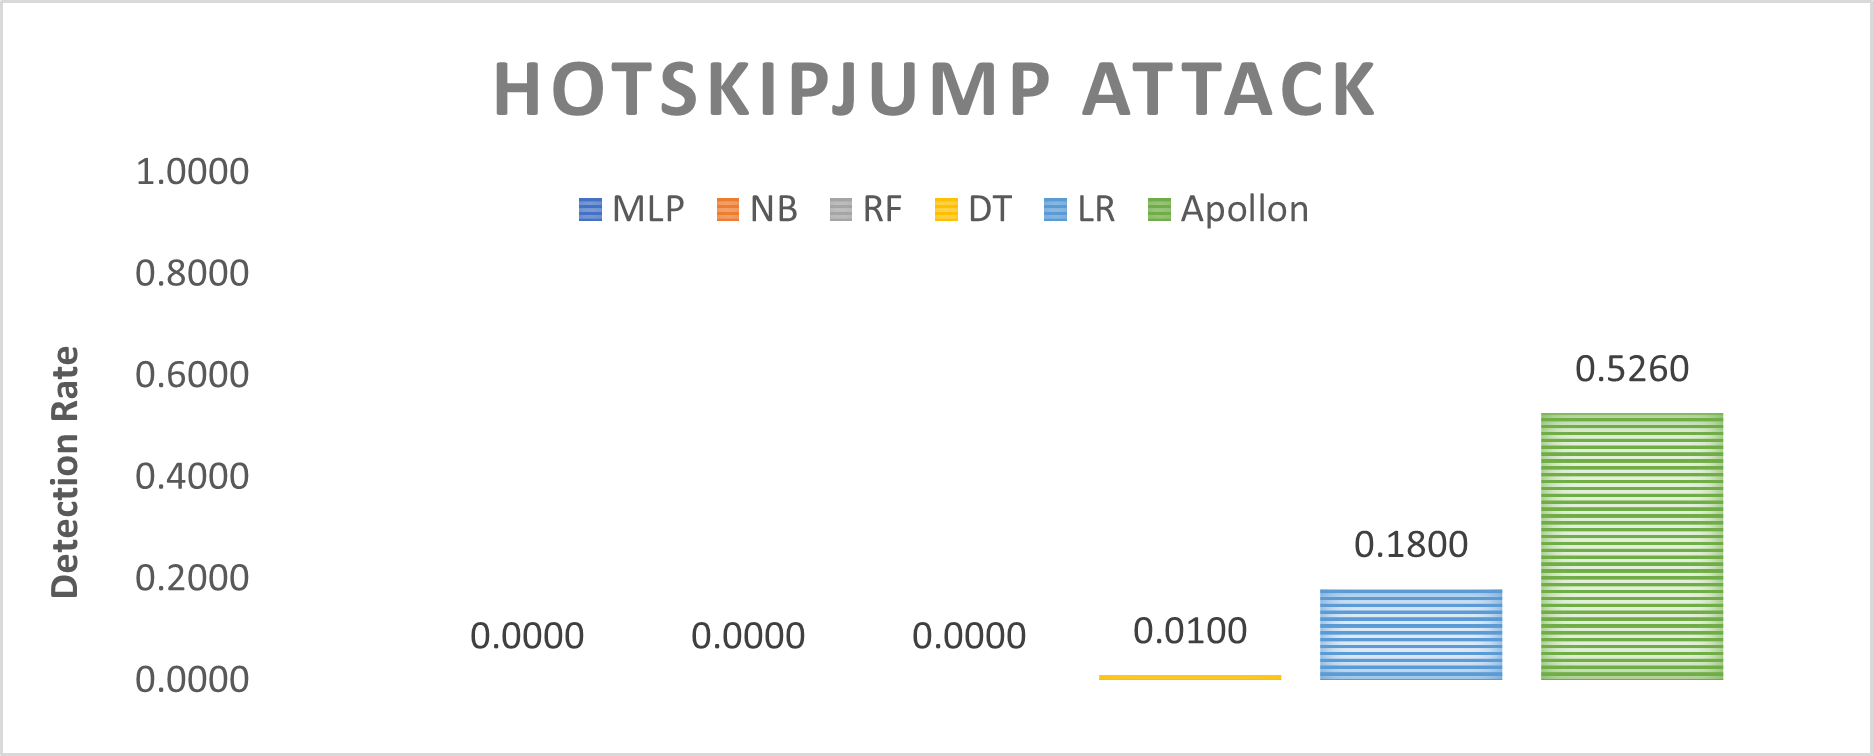
\includegraphics[width=0.9\columnwidth]{HSJA.png}
    \caption{\textit{HopSkipJump attack} Detection Rate results}
    \label{fig:hopskipjump-aml-results}
\end{figure}


Finally, the \textit{Wasserstein Generative Adversarial Network (W-GAN)} based attack was launched with a custom implementation
available in the \textit{Apollon} repository on GitHub.
This implementation was based on the \textit{IDSGAN} attack~\cite{lin2022idsgan}, apdated to the needs of the selected dataset.
The results in Table~\ref{tab:wgangp-aml-results} and in the Figure~\ref{fig:wgangp-aml-results} were obtained after
launching the attack with 100 epochs.

\begin{table}
    \centering
    \resizebox{\columnwidth}{!}{
        \begin{tabular}{l|llllll|}
            \cline{2-7}
                & \multicolumn{6}{c|}{\textbf{W-GAN based attack}} \\ \hline
            \multicolumn{1}{|l|}{Metrics} & \multicolumn{1}{c|}{MLP} & \multicolumn{1}{c|}{NB} & \multicolumn{1}{c|}{RF} & \multicolumn{1}{c|}{DT} & \multicolumn{1}{c|}{LR} & \multicolumn{1}{c|}{\textbf{Apollon}} \\ \hline
            \multicolumn{1}{|l|}{Accuracy} & 0.5002 & 0.4398 & 0.5001 & 0.4280 & 0.3230 & \textbf{0.6260} \\
            \multicolumn{1}{|l|}{Detection Rate} & 0.0000 & 0.0000 & 0.0000 & 0.0000 & 0.0000 & \textbf{0.4250} \\ \hline
        \end{tabular}
    }
    \caption{Results of the \textit{W-GAN} based AML attack}
    \label{tab:wgangp-aml-results}
\end{table}

\begin{figure}
    \centering
    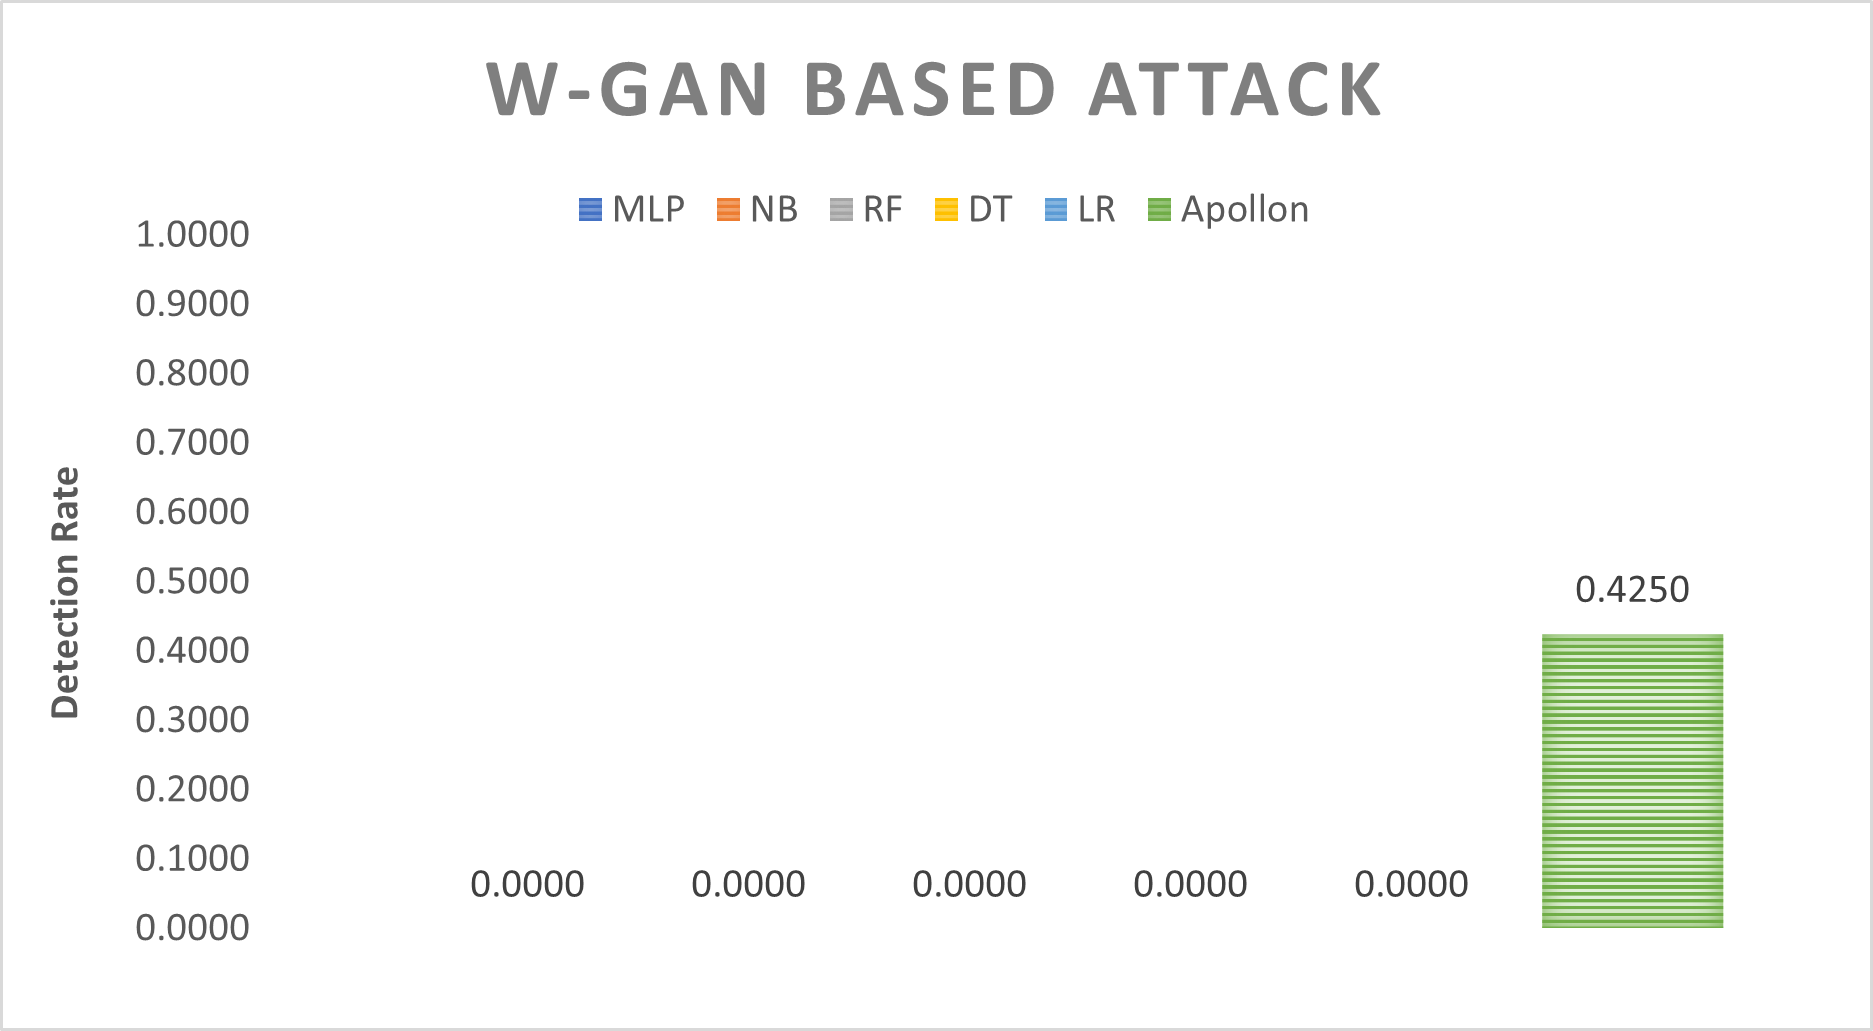
\includegraphics[width=0.9\columnwidth]{WGAN.png}
    \caption{\textit{W-GAN} based attack detection rate results}
    \label{fig:wgangp-aml-results}
\end{figure}

The \textit{W-GAN} based attack was the most effective attack, reducing the detection rate to zero in all the classifiers.
Our solution, on the other hand, was able to maintain a detection rate > 0.4.


\textit{Apollon}'s improved accuracy and detection rates in AML attacks can be attributed to the inclusion of an uncertainty
component in its model selection process.
This renders it difficult to train a model solely based on its responses.

The experimental results of the scenario reveals that our solution exhibits greater robustness in comparison to the
other classifiers used individually.

However, we also observed that while our solution effectively reduces the effectiveness of the attacks, it does not
completely nullify them.
This means that there is still room for improvement in terms of enhancing the solution's robustness to further strengthen
its resistance against such attacks.

In particular, if we were to generate the attacks with more time, such as by increasing the number of iterations or epochs,
it is likely that the effectiveness of these attacks against our solution would increase.